\documentclass[12pt]{article}
\setlength{\headheight}{14.5pt}
\addtolength{\topmargin}{-2.5pt}

\usepackage{cite}
\usepackage{pgfplots} % Add this line to include the pgfplots package
\usepackage{amsmath}
\usepackage{geometry}
\usepackage{setspace}
\usepackage{graphicx}
\usepackage{fancyhdr}
\usepackage{xcolor}
\usepackage{titlesec}
\usepackage{booktabs}
\usepackage{hyperref}
\usepackage{soul}
\usepackage{wrapfig}
\usepackage{placeins}
\usepackage{float}
\usepackage{amsmath}
 


\hypersetup{
    colorlinks=true,       % Enable colored links
    linkcolor=blue,        % Color of internal links
    filecolor=magenta,     % Color of file links
    urlcolor=cyan          % Color of external links
}



\renewcommand{\headrulewidth}{0pt} % Remove header rule
\renewcommand{\footrulewidth}{0pt} % Remove footer rule




\usepackage{url}
\geometry{a4paper, margin=0.7in }
\setlength{\parindent}{0pt}
\setstretch{1.5}
\headsep = 3pt %Move text closer to header
\usepackage{setspace}
% Header and Footer
\usepackage{fancyhdr}
\pagestyle{fancy}
\fancyhf{} % Clear all header and footer fields
\fancyhead[L]{\textbf{19-AIBM4}} % Top-left text

\renewcommand{\headrule}{\vspace{1pt}\hrule height 0.5pt} %Headrule spacing

% Optional: Adjust header line thickness if needed
\renewcommand{\headrulewidth}{0.5pt} % Thickness of the header line

% Combine the page numbering and horizontal rule into one footer definition
\fancyfoot[C]{\rule{\textwidth}{0.5pt}\\ Page \thepage\ of 15} % Bottom horizontal line with page number


% Title formatting
\titleformat{\section}[block]
  {\large\bfseries\sffamily\color{red}}
  {\thesection.}{1em}{}


\titleformat{\subsection}[block]
  {\normalsize\bfseries\sffamily\color{red}}
  {\thesubsection}{1em}{}
 \pgfplotsset{compat=1.18} 

 \titlespacing*{\subsection}{0pt}{1em}{0.2em}
 \titlespacing*{\section}{0pt}{1em}{0.5em}
\linespread{1.5}
\setlength{\abovedisplayskip}{0pt}
\setlength{\belowdisplayskip}{0pt}



\begin{document}


\pagenumbering{arabic} % Ensure Arabic numbering starts from the first page



 
% -------------------------------------------------------------
% COVER PAGE
% -------------------------------------------------------------
\begin{titlepage}
\centering
% University logo or other image

\includegraphics[width=0.4\textwidth]{UoD_Engineering.jpg} \\
\vspace{10mm}

% Title and subtitle
{\LARGE \textbf{Feasibility Report for Group 19-AIBM4 Autonomous Material Mover}} \\[10pt]

\vspace{5mm}\hrule\vspace{0mm}

% Insert image with caption for the material mover
\begin{figure}[h!]
    \centering
     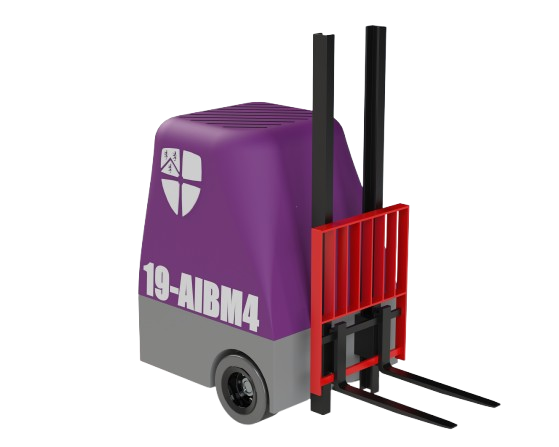
\includegraphics[width=1\textwidth]{Pooled_Design_V2__6_-removebg-preview.png}
\end{figure}  
\vspace{0mm}
\vspace{10mm}

% Title and author block
{\large \textbf{Co-Authors: }\textit{A Wright, A Wigmore, H Billing, J Wang, L Nangle, W Woodward}} \\ \vspace{1mm}
{Supervisors:\textit{ Dr Aissa Ikhlef, Bill Maxwell}} \\[10pt]
{\small Durham University \\ \today}
\end{titlepage}

% -------------------------------------------------------------
% FRONTMATTER
% -------------------------------------------------------------
\tableofcontents
%\begin{figure}[h!]
 %   \centering
 %    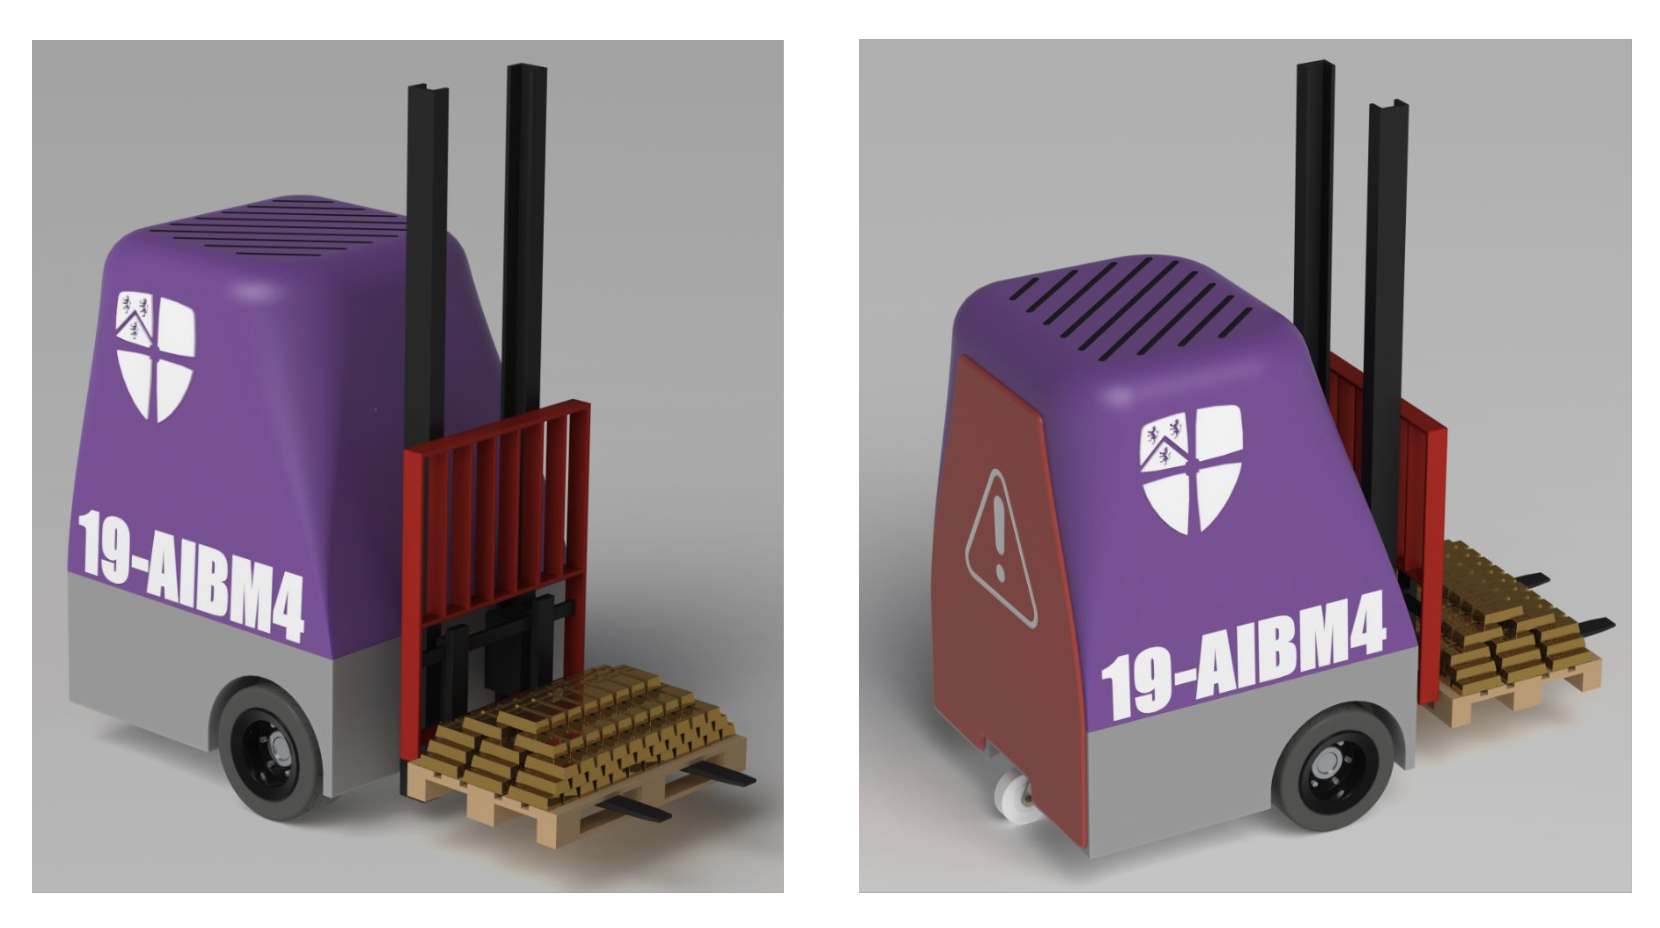
\includegraphics[width=0.65\textwidth]{finaldesign.png}
 %         \label{fig:final design}
%\end{figure}

\newpage

% -------------------------------------------------------------
% MAIN CONTENT
% -------------------------------------------------------------


% -------------------------------------------------------------
% 2. Introduction and Project Scope
% -------------------------------------------------------------
\section{Executive Summary}
This feasibility report looks into the development of an Automated Material Mover (AIBM4), which aims to transport materials autonomously within a factory environment. This would eliminate the need for manual handling of goods, improve productivity and ensure a safer and more sustainable working environment. 
\par Through an iterative design process, we chose a three-wheeled automated forklift design that integrates differential steering around a central axle for maximum manoeuvrability and tape sensing technology for precise movement within a factory environment. To make this design contemporary and sustainable, the body and forks will be made out of steel due to its high reconcilability, while the castor wheel will be made from a pre-consumer nylon, and we will use airless tyres to improve durability and reduce waste.
\par Engineering calculations validate the design's structural integrity and feasibility as well as ensuring compliance with ISO 3691-4  standards. An in-depth cost analysis demonstrates that this automated guided vehicles (AGVs) are financially viable over conventional manual forklifts, due to significant savings in labour and operating costs over time. A break even analysis determines that only 39 units need to be sold to generate a profit, this seems very achievable.
\par An adaptable factory layout design has been included which has been optimised for AGV operation, however the material mover has been designed to fit into the majority of modern-day factories. We have also conducted a risk assessment to mitigate any risks as well as created a Gantt chart which determines that the design process will be finished by the end of March 2025.
\par This report demonstrates the technical, economic and environmental upper hand that an automated material mover can be provide in a modern factory setting.

\section{Introduction}
\subsection{What is the problem that we are attempting to solve?}
Efficient material handling is essential in modern manufacturing, but conventional forklifts still require manual operation. This project seeks to eliminate manual dependency by designing an autonomous material mover.
 
\subsection{Issues with Conventional Manual Material Handling}

Manual labour and forklifts have several key issues within factory environments:

\begin{itemize}
    \item \textbf{Inefficiency:} Human workers require regular breaks, reducing productivity.
    \item \textbf{Safety concerns:} Human error can lead to an increased likelihood of an accident as well as a higher chance of injuries.
    \item \textbf{Cost:} Cost of labour is very large, and multiple shifts necessitates additional hiring costs.
    \item \textbf{Reliability:} Human error can lead to materials being moved to the wrong locations.
\end{itemize}

Overall, these issues reduce productivity and compromise workplace safety.


\section{Project Scope}
\begin{figure}[htbp]
    \centering
     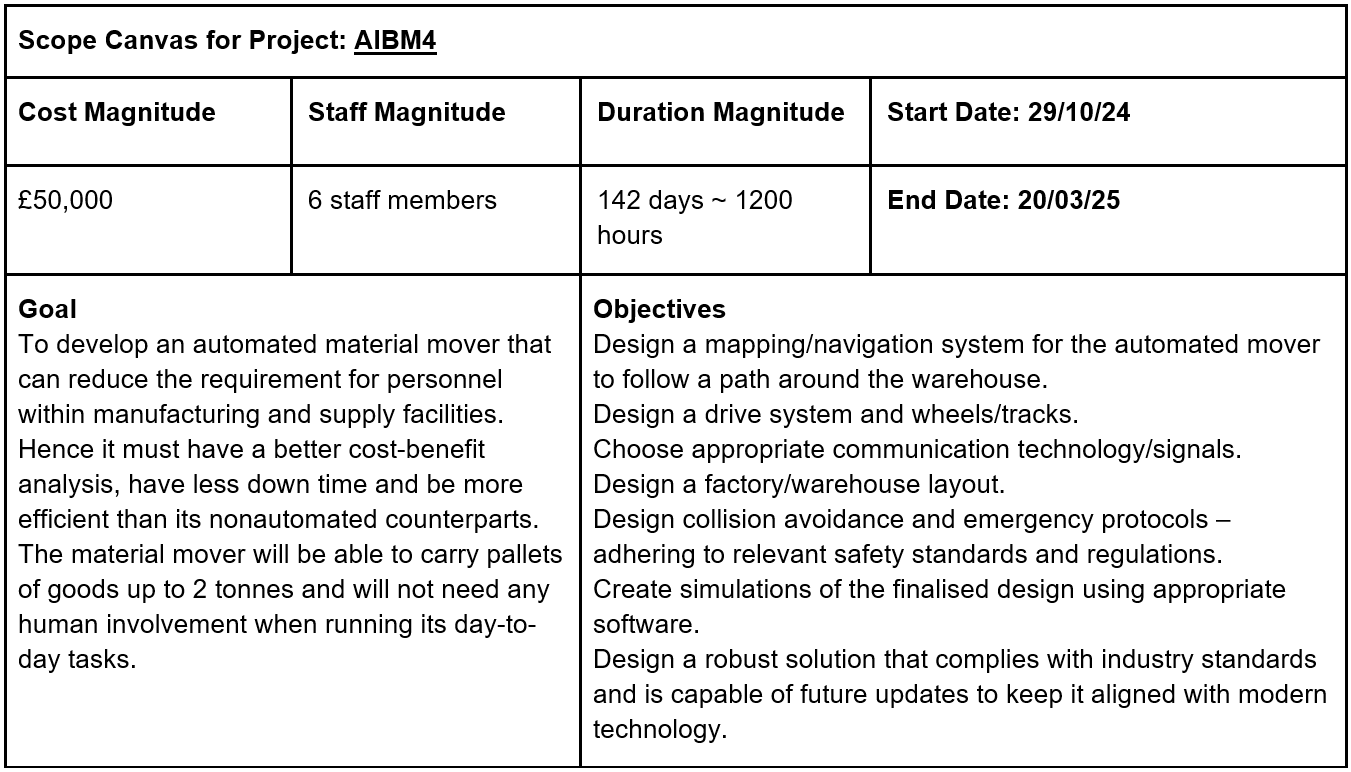
\includegraphics[width=0.9\textwidth]{Scope Canvas 1.png}
     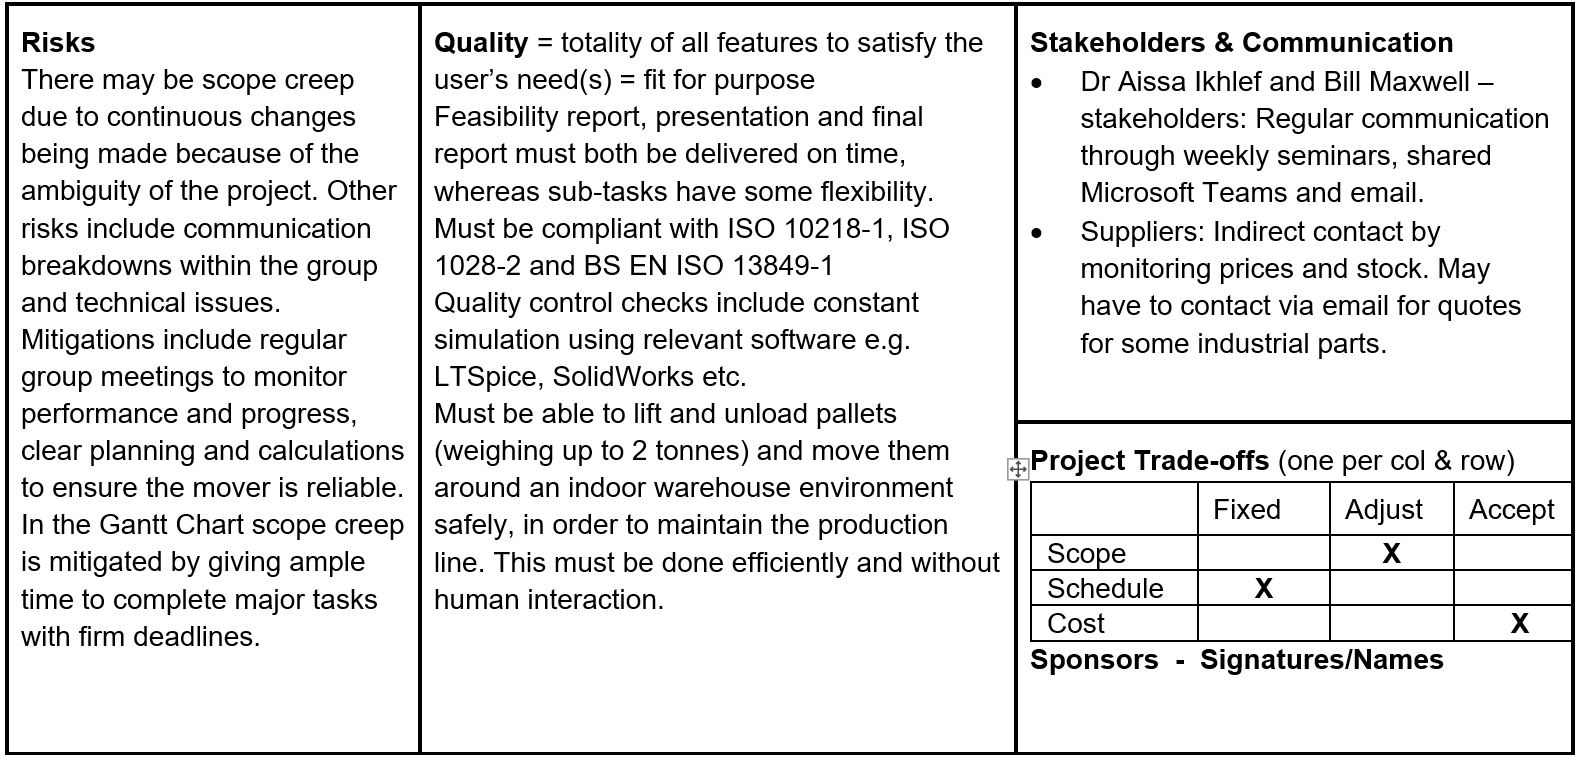
\includegraphics[width=0.9\textwidth]{Scope Canvas 2.png}
\end{figure}
\begin{figure}[htbp]
    \centering
     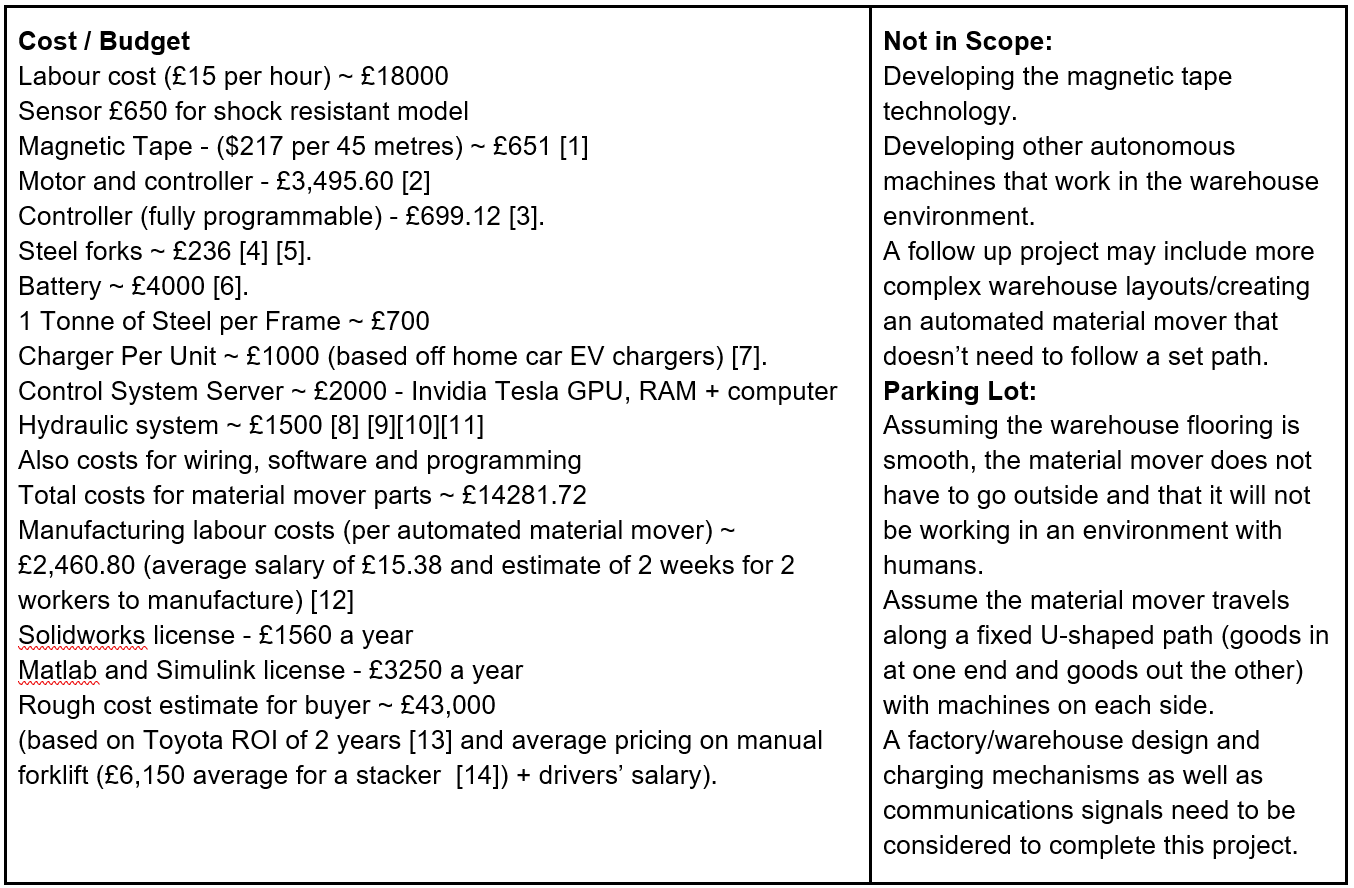
\includegraphics[width=0.9\textwidth]{Scope Canvas 3.png}
     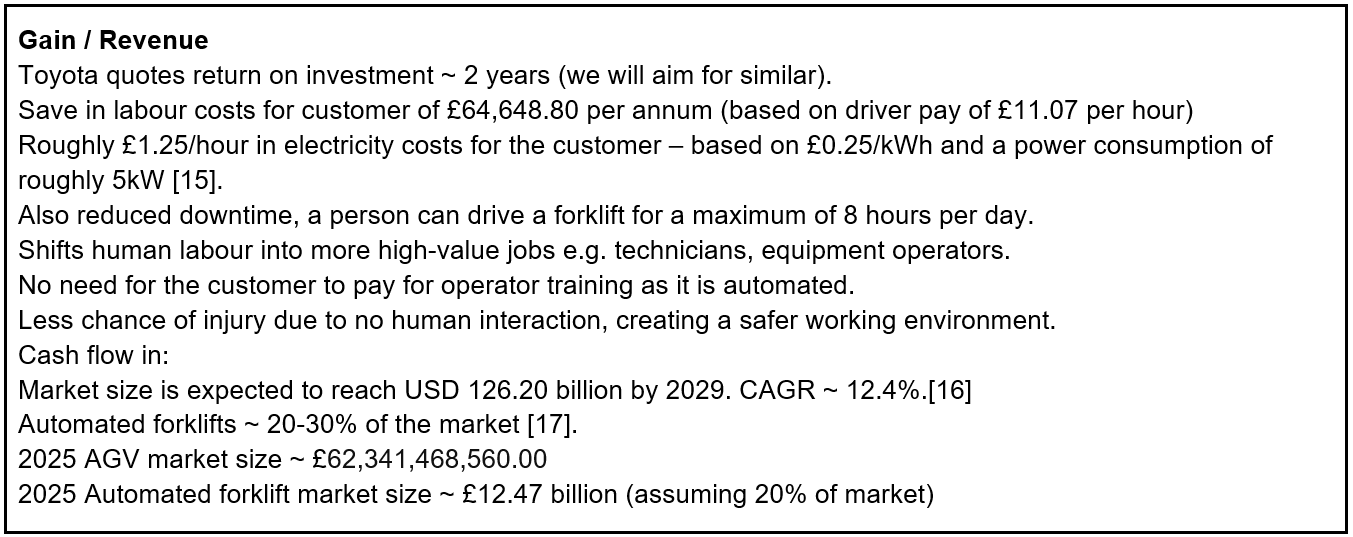
\includegraphics[width=0.9\textwidth]{Scope Canvas 4.png}
     \section{User-Requirement-Specification}
     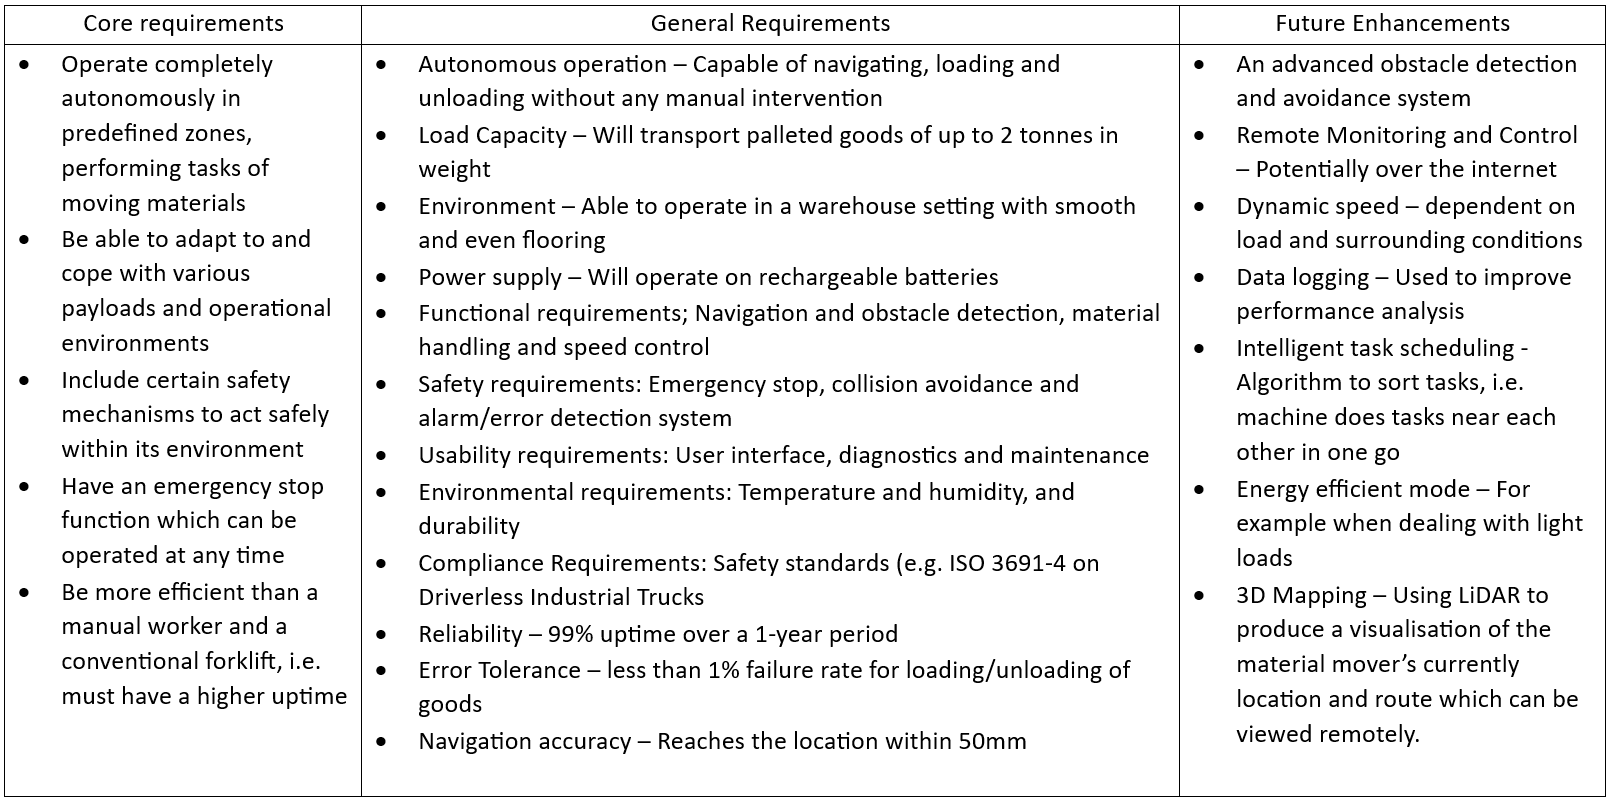
\includegraphics[width=0.9\textwidth]{URS1.png}
     \caption{URS – Automated Material Mover Project}
    \label{fig:URS}
\end{figure}

\FloatBarrier




% -------------------------------------------------------------
% 3. Concepts
% -------------------------------------------------------------
\section{Concepts}
\subsection{Possible Concepts}
 
\begin{enumerate}
    \item A three-wheeled mover with magnetic tape sensors. This design utilises a compact three wheeled configuration to allow for maximum manoeuvrability in tight spaces. Due to its magnetic tape sensing technology it can accurately navigate predefined paths within a factory setting and be easily integrated and changed within factories.
    \item A four-wheeled mover on a monorail. This design uses a monorail to ensure extremely precise movement as well as a four wheel base which makes it very sturdy for lifting goods and transporting them quickly and efficiently. An advantage of the design was that there was no down-time due to the material mover being constantly connected to a power source.
    \item A six-wheeled mover with line-following sensors. Six wheels allows for superior stability and load-bearing capabilities as well as maximum manoeuvrability. It would use differential steering for its central axis, with the other four wheels being caster wheels, to allow it to spin on the spot making it highly manoeuvrable and versatile.
 \end{enumerate}

 

\begin{figure}[h!]
    \centering
    % First image and its caption
    \begin{minipage}{0.32\textwidth}
        \centering
        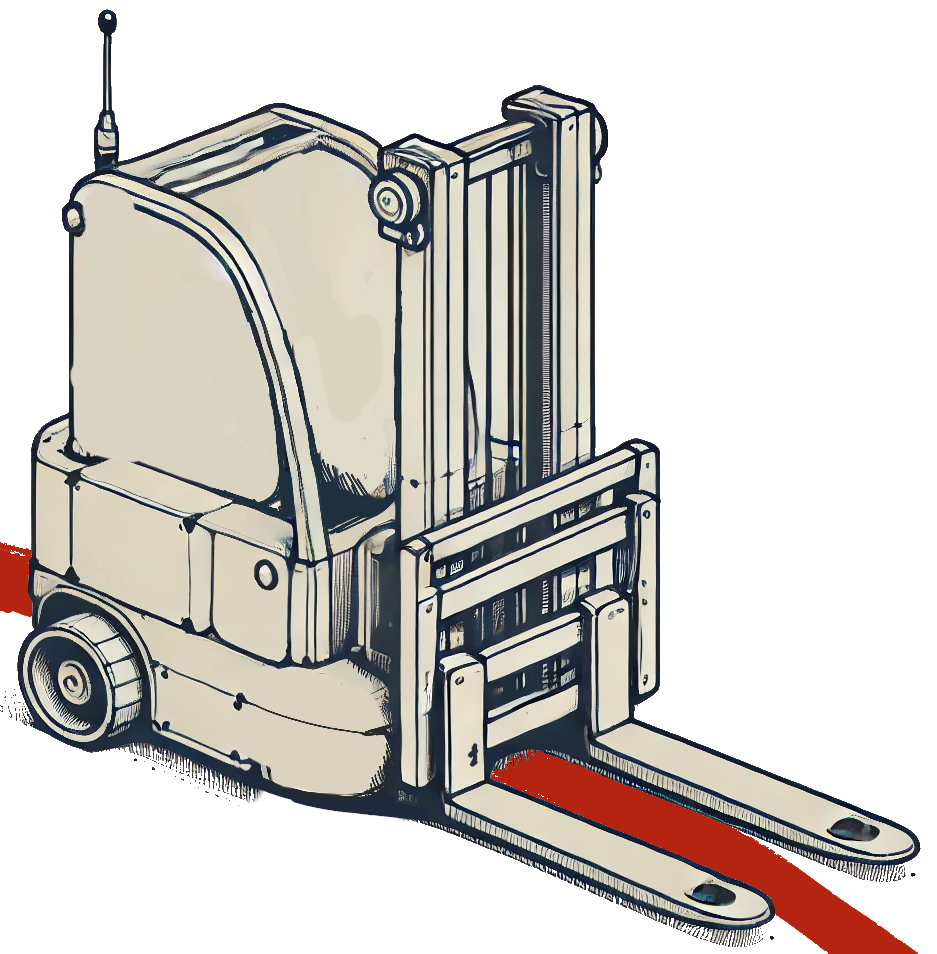
\includegraphics[width=\textwidth]{Simple_sketch_of_an_automated_forklift_robot_with_two_wheels_at_the_back_and_one_wheel_in_the_front.png}
    \end{minipage}%
    \hspace{0.01\textwidth}
    % Second image and its caption
    \begin{minipage}{0.32\textwidth}
        \centering
        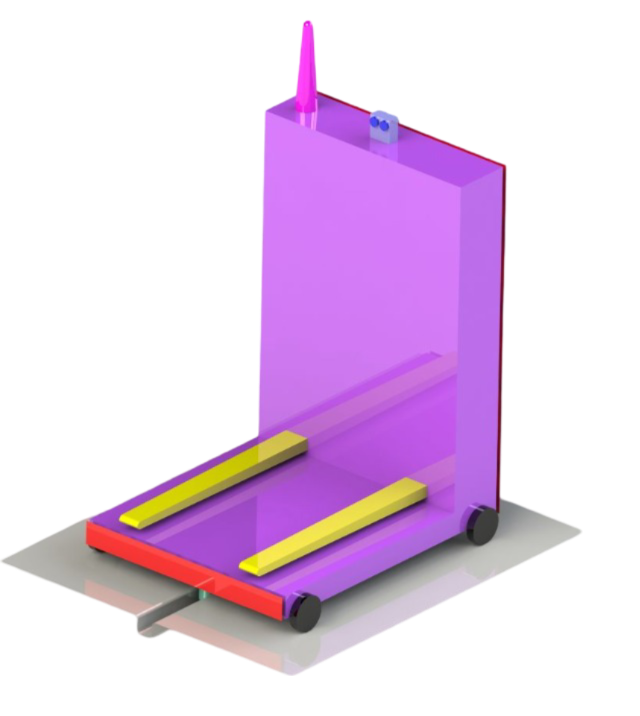
\includegraphics[width=\textwidth]{anna&will's design (1).png}
    \end{minipage}%
    \hspace{0.01\textwidth}
    % Third image and its caption
    \begin{minipage}{0.32\textwidth}
        \centering
        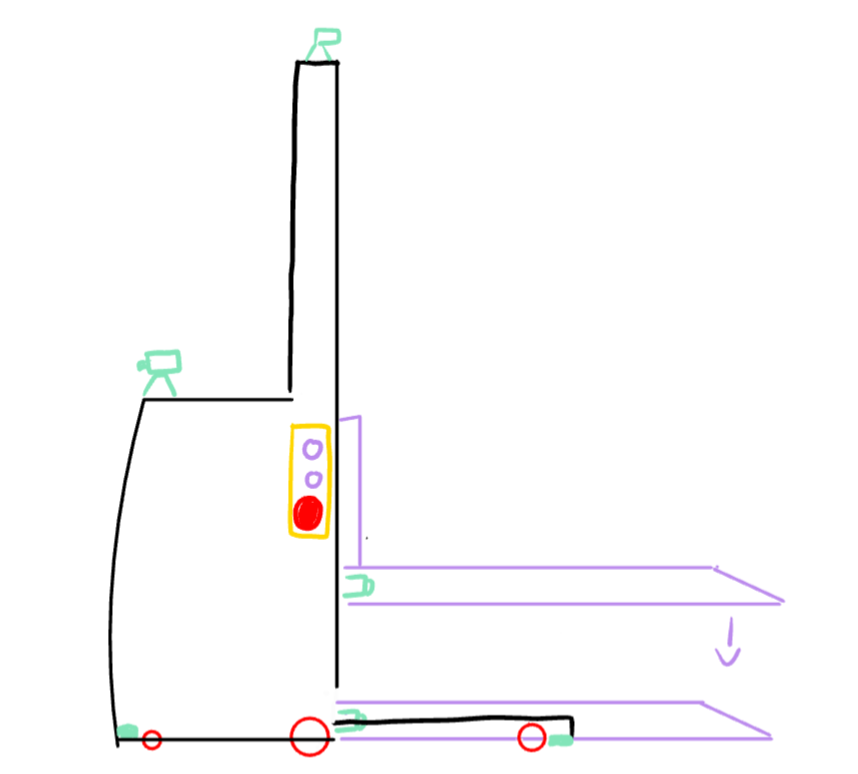
\includegraphics[width=\textwidth]{Louis' design without text.png}
    \end{minipage}
    \hspace{0.01\textwidth}
    
    % Captions below images
    \vspace{0.5mm}  % Adds space between the images and captions
    \begin{minipage}{0.32\textwidth}
        \centering
        \textbf{}Figure 2 (Concept 1): Three wheel magnetic tape following design
    \end{minipage}%
    \hspace{1.5mm} %Adds space between each caption
    \begin{minipage}{0.32\textwidth}
        \centering
        \textbf{}Figure 3 (Concept 2): Four wheel monorail design 
    \end{minipage}%
    \hspace{1.5mm} %Adds space between each caption
    \begin{minipage}{0.32\textwidth}
        \centering
        \textbf{}Figure 4 (Concept 3): Six wheel line following design  %%  better to use   \caption{Final design} for automation :D   \label{fig:final_design}
    \end{minipage}
\end{figure}
 

\subsection{Strengths and Weaknesses}
Each concept was evaluated against the URS using a design decision matrix. A summary of this is provided in Table \ref{tab:concept_evaluation} below.


\begin{table}[h!]
\centering
\caption{Concept Evaluation Matrix}
\begin{tabular}{@{}lccc@{}}
\toprule
\textbf{Criteria}      & \textbf{Concept 1} & \textbf{Concept 2} &\textbf{Concept 3} \\ \midrule
Load Capacity          & High               & Medium              & Medium            \\
Navigation Efficiency  & Medium             & High                & High              \\
Cost                   & Low                & Medium              & Medium            \\
Ease of Maintenance    & High               & Low                 & Low               \\ \bottomrule
\end{tabular}
\label{tab:concept_evaluation}
\end{table}
\FloatBarrier

 
\section{Chosen Solution}
\begin{figure}[ht]
    \centering
    \begin{minipage}[t]{0.27\textwidth}
        \vspace{0pt} 
        \centering
        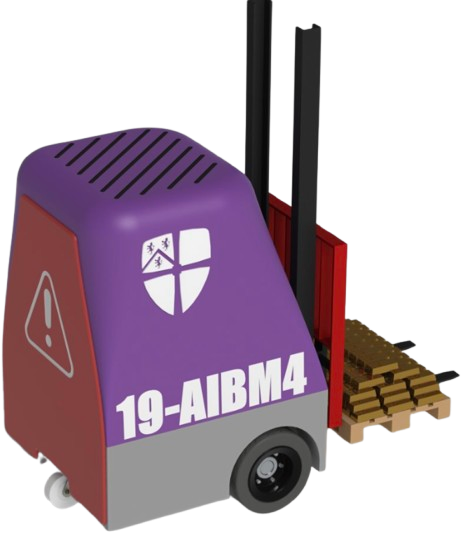
\includegraphics[width=\linewidth]{finaldesign1rb.png}  
        \vspace{-15pt}
        \caption{Final design}
        \label{fig:x}
    \end{minipage}%
    \hfill
    \begin{minipage}[t]{0.68\textwidth}
        \vspace{0pt}
        The initial design that was chosen was Concept one, with some changes to improve performance. For greater manoeuvrability, a counterweight design was chosen, removing the frontmost wheels to allow the lifter to rotate about its centre. In order to improve sustainability, the body and forks are likely to be made from steel because it has the highest recycling rate among all materials used in construction and engineering \cite{baker2023}. The castor wheels can be made of high-quality pre-consumer nylon (from the waste of polyester production) \cite{eco2022} and the drive wheels can be airless tires, as this would reduce the amount of rubber that goes into landfill and improve fuel efficiency \cite{ImperialTyres}. The design will be guided by two magnetic tape sensors which can follow a line of magnetic tape on the floor.
    \end{minipage}
\end{figure}




\subsection {Stress and Deflection Calculations}
\begin{figure}[H]
    \centering
    \begin{minipage}[t]{0.5\textwidth}
        \vspace{0pt}
        \linespread{1.5}
        Assuming the fork is a beam of uniform cross section fixed at the left end to the forklift, it can be modelled as shown in Figure \ref{fig:x}. This calculation uses a factor of safety of three for the maximum load, as specified by ISO 2330 for the prototyping of forklift forks \cite{iso2330}.
    \end{minipage}%
    \hfill
    \begin{minipage}[t]{0.45\textwidth}
        \vspace{-32pt} 
        \centering
        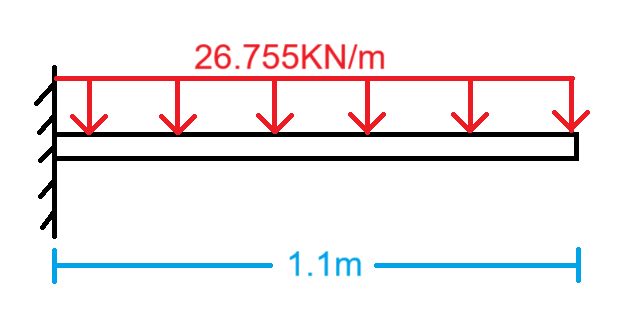
\includegraphics[width=\linewidth]{fork as a beam diagram.png}
        \vspace{-40pt}
        \caption{Diagram showing the force diagram of a singular fork.}
        \label{fig:x}
    \end{minipage}
\end{figure}


Using Macauley's method, the equation for the deflection of a steel-304 fork with \( E = 190 \, \text{GPa} \), height \( h = 40 \, \text{mm} \), and width \( b = 100 \, \text{mm} \cite{ForkDimensions} \) is given by:


\vspace{-20pt}
\begin{equation}
   \nu = \frac{3}{304000} \left( \frac{-16186.5}{2}x^2 + \frac{29430}{6}x^3 - \frac{26755}{24}x^4 \right)
\end{equation}
\vspace{-20pt}

Therefore maximum deflection is at \(x = 1.1 \, \text{m}\), which is \(\nu = -4.83 \, \text{cm}\).
For fatigue, following ISO-2330 standards a cyclic stress amplitude of 1.655MPa was obtained using equation (2).

\vspace{-20pt}
\begin{equation}
   \text{Cyclic Stress Amplitude} = \left (\frac{Force}{Area} \right)
\end{equation}
\vspace{-20pt}

The obtained value is smaller than the minimum fatigue limit of \(175 \text{MPa}\) so no cracking due to fatigue will occur.


\subsection{Centre of Mass calculations}

\begin{figure}[H]
    \centering
    \begin{minipage}[t]{0.57\textwidth}
        \vspace{0pt} % Align top of this minipage with the other
        In a counterbalance forklift design, tipping is avoided by using a counterbalance to shift the centre of mass to in between the wheels. The mover will tip about the drive wheel when the force through the rear wheel \( F_r = 0 \) and the load moment is greater than the counterbalance moment. The wheelbase is the distance between the drive and rear wheel, and \( Y \) shows the distance from the drive wheel to the centre of mass of the forklift. 
    \end{minipage}%
    \hfill
    \begin{minipage}[t]{0.38\textwidth}
        \vspace{-30pt} 
        \centering
        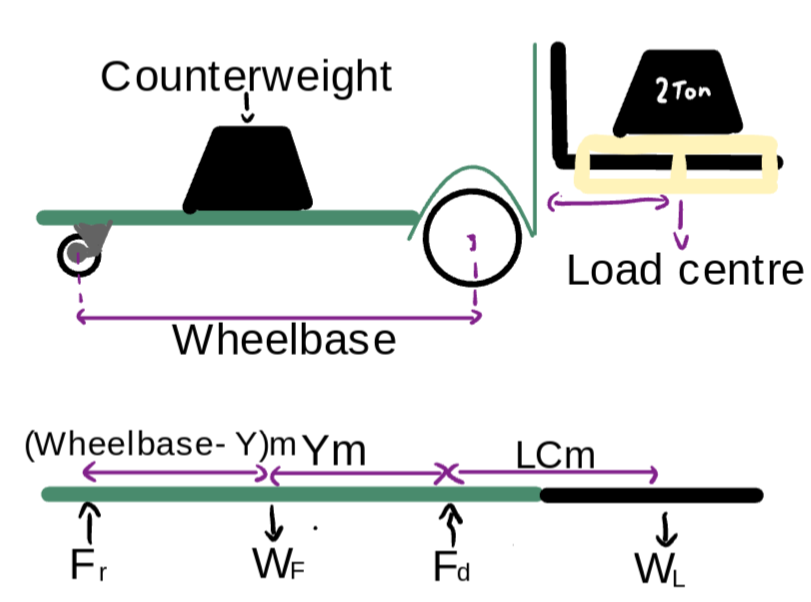
\includegraphics[width=\linewidth]{Tipping Calculations 3.png}
        \vspace{-30pt}
        \caption{Diagram of forklift mass distribution, and free body diagram}
        \label{fig:x}
    \end{minipage}
\end{figure}
The weight of the whole forklift is shown as \(W_F\) and the weight of the load is \(W_L\) acting at a distance equal to the load centre \(LC\) from the drive wheel. Taking moments about the drive wheel gives the following equation:
\vspace{-10pt}
\begin{equation}
    W_{\text{F}}Ym = W_{\text{L(tip)}}LCm
\end{equation}
\vspace{-35pt}

The Toyota 06-8FG20F \cite{Toyota} offers an example of a similar manual forklift with the same load ratings as our design. In this model, the counterweight has a mass of 4318kg, which gives a load tipping weight of 3750 kg, and a factor of safety against tipping of 1.875. This gives us an aim for a value that ensures our forklift is safe, but does not compromise efficiency through unnecessary added weight. Shifting the  counterweight further back would be a good way of reducing the necessary counterweight mass. Further safety features such as load sensors would further increase the safety of our design.

\subsection{Motor Torque Calculation}

The total drive force the vehicle needs is the sum of rolling resistance, air resistance, other smaller resistive forces such as resistance in the bearings and motor, and accelerating force. For the purposes of these calculations, the vehicle is assumed to need to reach a top speed of $8mph$ ($3.58ms^{-1}$), in a time of up to $5s$, similar other forklifts[SRC], and since the speed is relativity low, air resistance is assumed to be negligible. Rolling resistance, $F_{rr}$, is given by:
\vspace{-20pt}
\begin{equation}
    F_{rr} = C_{rr} m g = 0.015 \times 5000 \times 9.81 =  735.8 \, \text{N}
\end{equation}
\vspace{-40pt}

Where \( C_{rr} \) = Coefficient of Rolling Resistance, taken for tyres on concrete to be 0.015[SRC] \cite{RollingResistance}, \( m \) = Mass of the vehicle, taken to be \( 5000 \, \text{kg} \) as previously calculated[SRC], and \( g \) = Acceleration due to gravity, taken to be \( 9.81 \, \text{ms}^{-2} \). The accelerating force, \( F_a \), is given by:
\vspace{-20pt}
\begin{equation}
    F_a = m\frac{\Delta v}{\Delta t} = 5000\times \frac{3.58}{5} = 3580 \, \text{N}
\end{equation}


Where $\Delta v$ = Required change in speed, taken as the top speed of $3.58ms^{-1}$, and $\Delta t$ = Time to execute required speed change, taken as $5s$. And so the total drive force required is the sum of these forces,
\vspace{-5pt}
\begin{equation}
    F_d = F_{rr} + F_a = 735.8 \, + \, 3580 = 4315.8 \, \text{N}
\end{equation}
\vspace{-40pt}

The motor torque required to produce this force, $T_m$, is given by:
\vspace{-20pt}
\begin{equation}
    T_m = F_d \times R_w \times RF = 4315.8 \times 0.289 \times 1.15 = 2.228 \, \text{kNm}
\end{equation}
\vspace{-40pt}

Where $R_w$ = Wheel radius, valued at $0.289m$, and RF = Resistance Factor, which accounts for smaller resistances such as those in the bearing and the motor, and is taken as 1.15. Therefore, if each motor is picked to have 2.5kNm of torque, the total drive torque will be 5kNm - over twice what is required, ensuring that the vehicle has sufficient torque.






\subsection {Hand Calculations}
\begin{figure}[H]
    \centering
    \begin{minipage}[t]{0.5\textwidth}
        \vspace{0pt}
        \linespread{1.5}
        Assuming the fork is a beam of uniform cross section fixed at the left end to the forklift, it can be modelled as shown in Figure \ref{fig:x}. This calculation uses a factor of safety of three for the maximum load, as specified by ISO 2330 for the prototyping of forklift forks \cite{iso2330}.
    \end{minipage}%
    \hfill
    \begin{minipage}[t]{0.45\textwidth}
        \vspace{-32pt} 
        \centering
        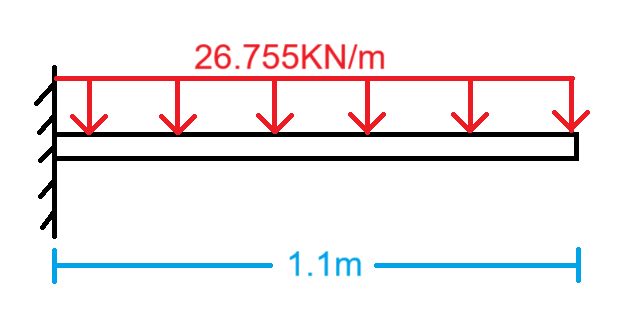
\includegraphics[width=\linewidth]{fork as a beam diagram.png}
        \vspace{-40pt}
        \caption{Diagram showing the force diagram of a singular fork.}
        \label{fig:x}
    \end{minipage}
\end{figure}


Using Macauley's method, the equation for the deflection of a EN19 steel fork with \( E = 200 \, \text{GPa} \), height \( h = 40 \, \text{mm} \), and width \( b = 100 \, \text{mm} \cite{ForkDimensions} \) is given by:

\vspace{-20pt}
\begin{equation}
   \nu = \frac{3}{320000} \left( \frac{-16186.5}{2}x^2 + \frac{29430}{6}x^3 - \frac{26755}{24}x^4 \right)
\end{equation}
\vspace{-20pt}

Therefore the maximum deflection, at the furthest point from the fork's support, \(x = 1.1 \, \text{m}\), is \(\nu = -45.9mm \, \text{mm}\).
For fatigue, following ISO-2330 standards a cyclic stress amplitude of 1.655MPa was obtained using equation (2).

\vspace{-20pt}
\begin{equation}
   \text{Cyclic Stress Amplitude} = \left (\frac{Force}{Area} \right)
\end{equation}
\vspace{-20pt}

The obtained value is smaller than the minimum fatigue limit of \(175 \text{MPa}\) so no cracking due to fatigue will occur.

\begin{figure}[H]
    \centering
    \begin{minipage}[t]{0.57\textwidth}
        \vspace{0pt} % Align top of this minipage with the other
        In a counterbalance forklift design, tipping is avoided by using a counterbalance to shift the centre of mass behind the drive wheels. The mover will tip about the drive wheel when the force through the the load moment is greater than the counterbalance moment. The wheelbase is the distance between the drive and rear wheel, and \( Y \) shows the distance from the drive wheel to the centre of mass of the forklift. 
    \end{minipage}%
    \hfill
    \begin{minipage}[t]{0.38\textwidth}
        \vspace{-30pt} 
        \centering
        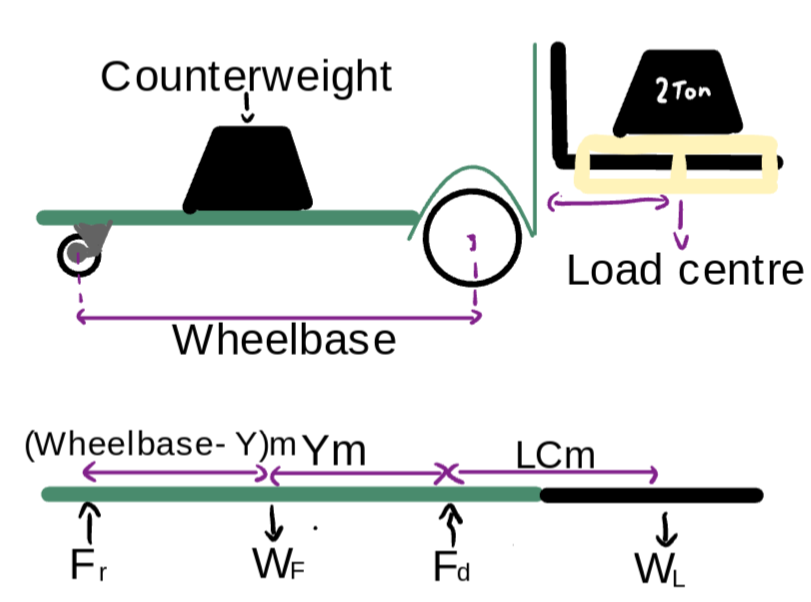
\includegraphics[width=\linewidth]{Tipping Calculations 3.png}
        \vspace{-30pt}
        \caption{Diagram of forklift mass distribution, and free body diagram}
        \label{fig:x}
    \end{minipage}
\end{figure}
The weight of the whole forklift is shown as \(W_F\) and the weight of the load is \(W_L\) acting at a distance equal to the load centre \(LC\) from the drive wheel. Knowing that at the point of tipping, $F_r = 0N$ and taking moments about the drive wheel:
\vspace{-10pt}
\begin{equation}
    W_{\text{F}}Y = W_{\text{L(tip)}}LC
\end{equation}
\vspace{-35pt}

Not a fan of m and Cm not being units when distance is involved, kinda confusing

The Toyota 06-8FG20F \cite{Toyota} offers an example of a similar manual forklift with the same load ratings as our design. In this model, the counterweight has a mass of 4318kg, which gives a load tipping weight of 3750 kg, and a factor of safety against tipping of 1.875. Our design takes $LCm$ as $0.967m$, $Ym$ as $1m$, $W_L$ as $3750gN$ (a 2 tonne load multiplied by the 1.875 factor of safety), and so determines that:

\vspace{-10pt}
\begin{equation}
    W_{\text{F}} = \frac{W_{\text{L(tip)}}LCm}{Ym} = \frac{3750g \times 0.967}{1} = 3626.25gN
\end{equation}
\vspace{-35pt}

This means a counterweight of 3626kg - similar to the value Toyota use. For the sake of saftey and simplicity in further calculations, this value will be rounded up to 4000kg. This gives us an aim for a value that ensures our forklift is safe, but does not compromise efficiency through unnecessary added weight. Shifting the  counterweight further back would be a good way of reducing the necessary counterweight mass. Integrating load sensors would ensure that the 2 tonne limit is not exceeded, preventing damage to the forklift.

The weight of the forklift is an important factor in the driving force that it requires. The total drive force the vehicle needs is the sum of rolling resistance, air resistance, other smaller resistive forces such as resistance in the bearings and motor, and accelerating force. For the purposes of these calculations, the vehicle is assumed to need to reach a top speed of $8mph$ ($3.58ms^{-1}$), in a time of up to $3s$, similar other forklifts[SRC], and since the speed is relativity low, air resistance is assumed to be negligible. Rolling resistance, $F_{rr}$, is given by:
\vspace{-20pt}
\begin{equation}
    F_{rr} = C_{rr} m g = 0.015 \times 6000 \times 9.81 =  882.9 \, \text{N}
\end{equation}
%\vspace{-40pt}

Where \( C_{rr} \) = Coefficient of Rolling Resistance, taken for tyres on concrete to be 0.015[SRC] \cite{RollingResistance}, \( m \) = Mass of the vehicle, taken to be \( 6000 \, \text{kg} \) as previously calculated plus the load weight[SRC], and \( g \) = Acceleration due to gravity, taken to be \( 9.81 \, \text{ms}^{-2} \). The accelerating force, \( F_a \), is given by:
\vspace{-20pt}
\begin{equation}
    F_a = m\frac{\Delta v}{\Delta t} = 6000\times \frac{3.58}{3} = 7160 \, \text{N}
\end{equation}


Where $\Delta v$ = Required change in speed, taken as the top speed of $3.58ms^{-1}$, and $\Delta t$ = Time to execute required speed change, taken as $5s$. And so the total drive force required is the sum of these forces,
\vspace{-5pt}
\begin{equation}
    F_d = F_{rr} + F_a = 882.9 \, + \, 7160 = 8042.9 \, \text{N}
\end{equation}
\vspace{-40pt}

The motor torque required to produce this force, $T_m$, is given by:
\vspace{-20pt}
\begin{equation}
    T_m = F_d \times R_w \times RF = 8042.9 \times 0.289 \times 1.15 = 2.673 \, \text{kNm}
\end{equation}
\vspace{-40pt}

Where $R_w$ = Wheel radius, valued at $0.289m$, and RF = Resistance Factor, which accounts for smaller resistances such as those in the bearing and the motor, and is taken as 1.15. Therefore, if each motor is picked to have 2.5kNm of torque, the total drive torque will be 5kNm - roughly twice what is required, ensuring that the vehicle has sufficient torque.

\subsection{Expected Cost}

\begin{table}[H]
    \centering
    \begin{minipage}[t]{0.5\textwidth}
        \setlength{\parskip}{0pt} % No extra space between paragraphs
        \vspace{-10pt}
        The estimated cost of the product \cite{P. Hinz} is £60,000, and this covers:
        \begin{itemize}
        \setlength{\itemsep}{1pt}
            \item All the hardware for the autonomous material mover
            \item All of the software acquisition and development for navigation, and task automation.
            \item The implementation of the system into a conventional factory; however, this will likely differ on a site-to-site basis.
        \end{itemize}
    \end{minipage}%
    \hfill
    \begin{minipage}[t]{0.45\textwidth}
        \centering
        \vspace{-10pt}
        \begin{tabular}{|l|r|}
            \hline
            \textbf{Cost Item}          & \textbf{Amount (£)} \\ \hline
            Labour Costs                 & 18,000.00           \\ \hline
            Material Costs              & 15,099.12           \\ \hline
            Overheads                   & 10,000.00           \\ \hline
            Software and Simulation     & 2,000.00            \\ \hline
            Contingency                 & 4,900.88            \\ \hline
            \textbf{Total Estimated Cost} & \textbf{60,000.00}  \\ \hline
        \end{tabular}
        \vspace{1pt} 
        \caption{Breakdown of Expected Costs for the Autonomous Material Mover}
        \label{tab:expected_costs}
    \end{minipage}
\end{table}



\begin{figure}[ht]
    \centering
    \begin{minipage}{0.45\linewidth}
        \centering
        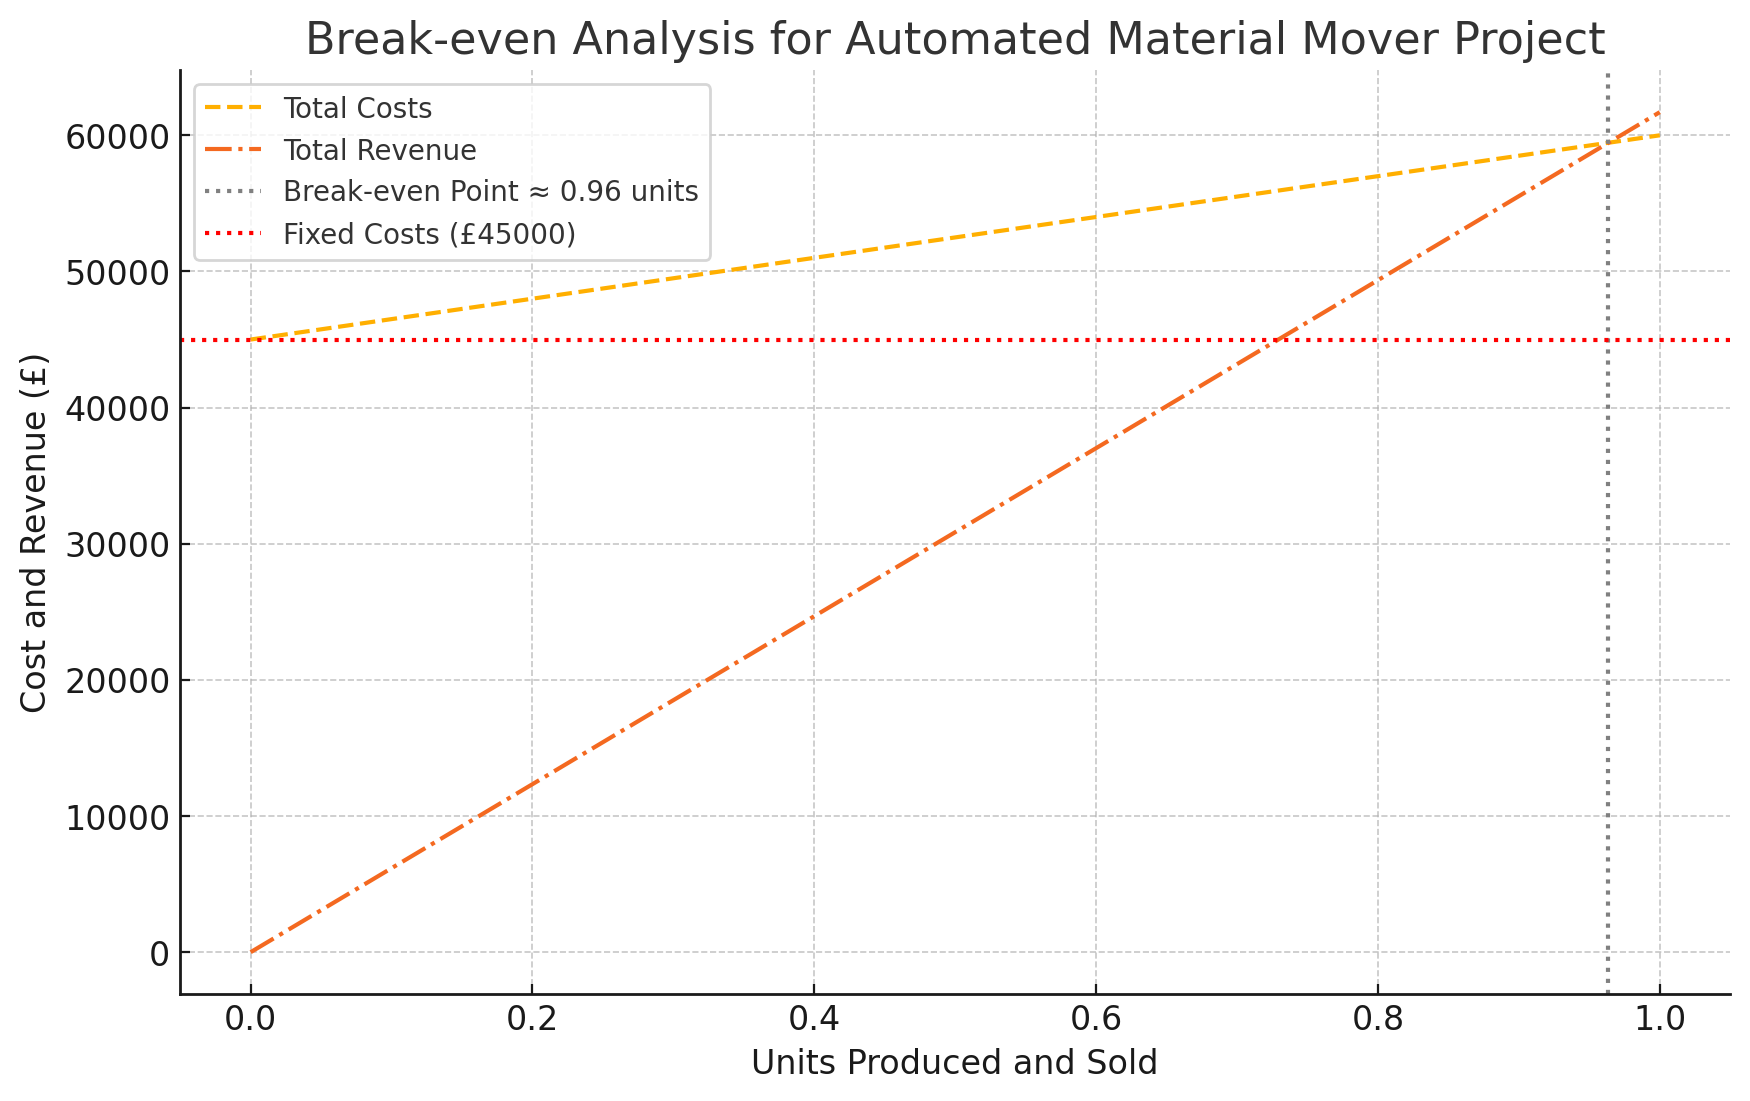
\includegraphics[width=\linewidth]{breakeven.png} % Replace with your Blender animation image
        \caption{Breakeven Point Analysis}
        \label{fig:breakeven}
    \end{minipage}
    \hspace{0.05\linewidth}
    \begin{minipage}{0.45\linewidth}
        \centering
        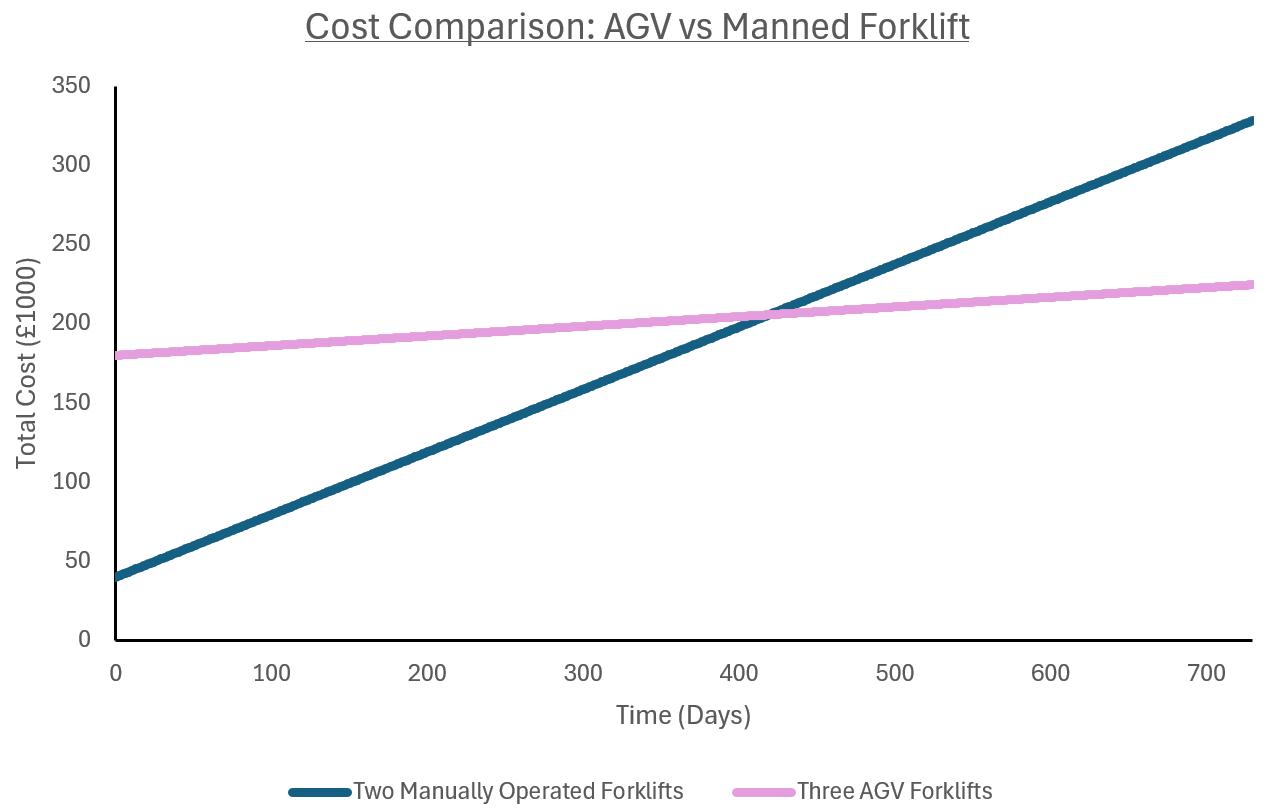
\includegraphics[width=\linewidth]{CostComparison1.png}
        \caption{Cost Comparison: AGVs vs Manned Forklift}
        \label{fig:timeline}
    \end{minipage}
\end{figure}


\FloatBarrier
\subsection{Cost Comparison for a Customer}
Whilst this product may seem expensive at first to potential customers, it has distinct financial and logistical advantages over manual forklifts. 
It should be considered that automated forklifts do, on average, move slower than regular manually driven forklifts. This means that it takes around 1.3-1.5 automated forklifts to do the same work as a single manned truck \cite{Pastor-Tella2024}. 
Taking these things into consideration, the following table assumes a factory using two manned forklifts, and how these costs would compare to three AGVs.
 
\begin{table}[htbp]
\centering
\begin{tabular}{|l|l|l|}
\hline
\textbf{Cost Factor}                   & \textbf{Manual Forklifts}           & \textbf{AGVs } \\ \hline
\textbf{Initial Cost per Unit}          & £20,000                             & £60,000                               \\ \hline
\textbf{Number of Units}                & 2                                    & 3                                     \\ \hline
\textbf{Total Initial Cost}             & 2 × £20,000 = £40,000               & £180,000                \\ \hline
\textbf{Annual labour cost per forklift }& £11.44× 16×365 = £66,810      & £0                                    \\ \hline
\textbf{Total Annual Labor Cost (16 hours a day)}        & 2 x £66,810 = £129,297.6    & £0                                    \\ \hline
 \textbf{Electricity cost per year (25.46p per kWh) } & £14,868&£22,302\\\hline  
 
\textbf{Total Annual Operating Cost}    & £148,487& £22,302\\ \hline
 
  
\end{tabular}

\caption{Cost Breakdown for Manual and Automated Forklifts}
\end{table}

\FloatBarrier
Cost per unit taken as £60,000 for an AGV, compared with £20,000 for a manual forklift. From the graph in Figure 8 we can see that after 420 days of operation the three AGV forklifts become more economical in comparison to the two manually operated forklifts. 
\FloatBarrier
\subsection{Factory Layout}

 \FloatBarrier
A CAD factory layout has been produced using information from EG Propertylink listing for Unit 5, Hurworth Road, Aycliffe Business Park \cite{mileway_hurworth_2024} as an example. This layout makes use of a U shaped path for the movers, with  machines along either side of the path. The path is marked with magnetic tape which the movers can detect and follow using sensors. At each end  of the path will be the goods in and goods out areas, where the movers will collect supplies for the machines and deposit finished products respectively. In these areas there will also be charging stations, positioned out of the way to prevent disruption.
\begin{figure}[ht]


        \centering
        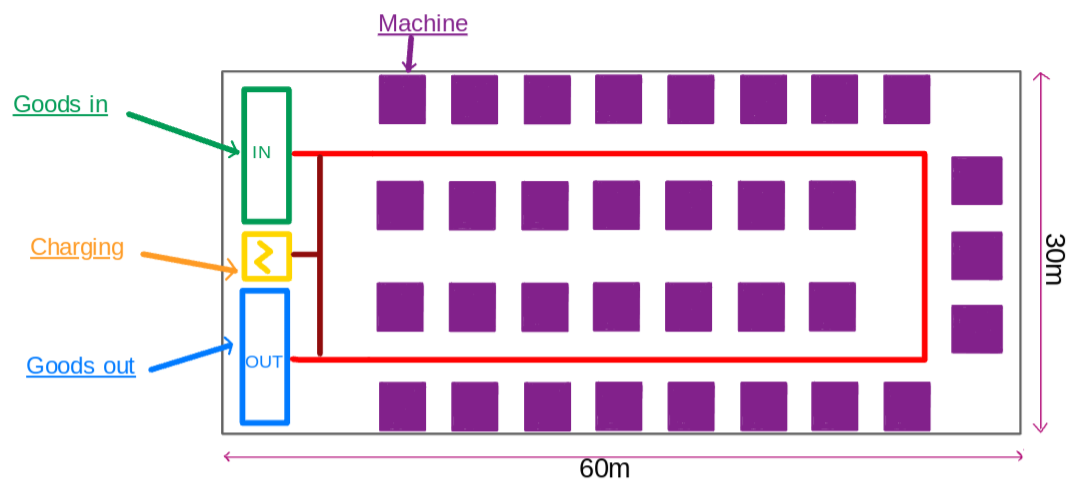
\includegraphics[width=0.8\linewidth]{Factory Layout Louis Big Text.png}
        \caption{Factory design layout}
        \label{fig:factory_layout}

\end{figure}
\FloatBarrier
 

 
\begin{figure}[h!]
 \section{Risk assessment }
    \centering
    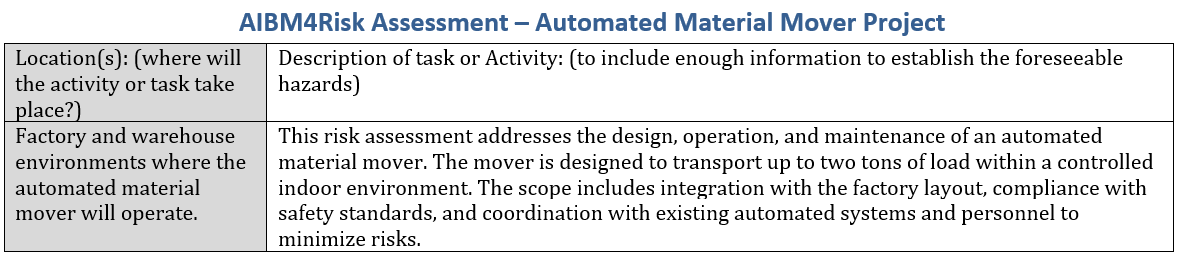
\includegraphics[width=0.85\textwidth]{Risk1.png}
    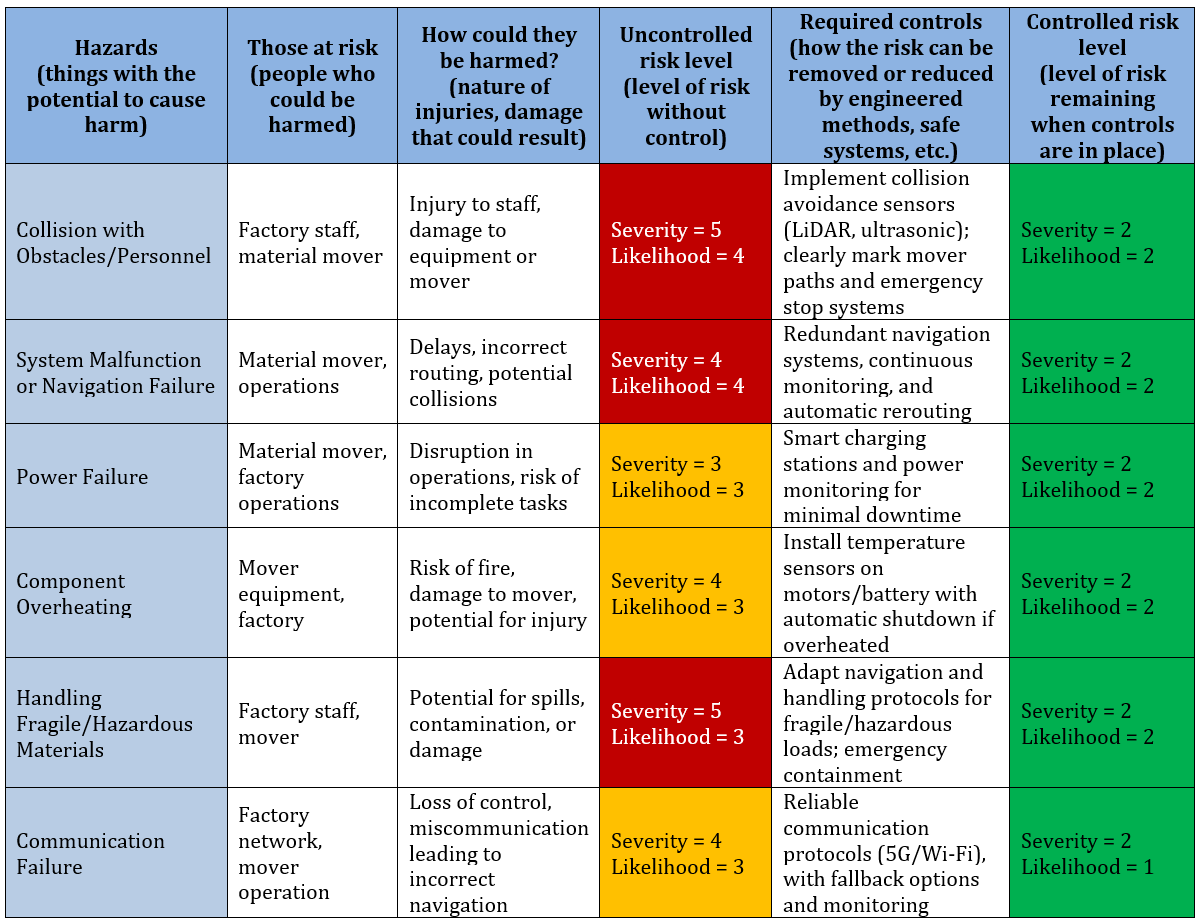
\includegraphics[width=0.85\textwidth]{Risk2.png}
\end{figure}
\begin{figure}[h!]
    \centering
    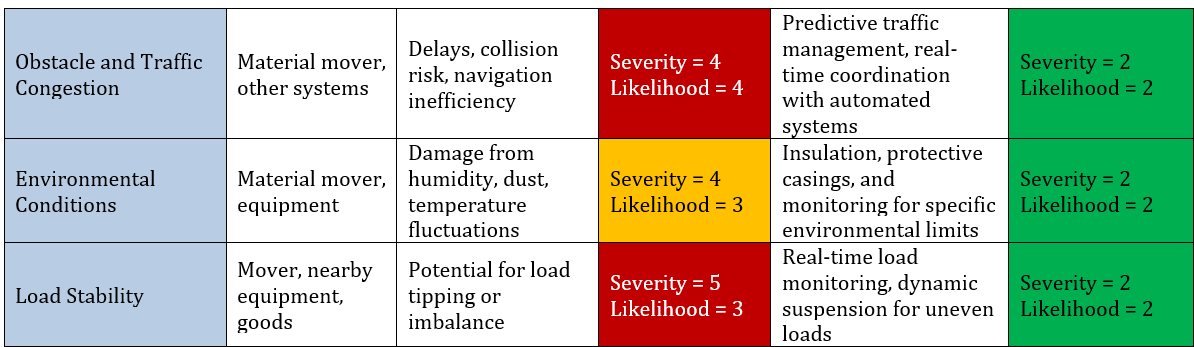
\includegraphics[width=0.85\textwidth]{Risk3.png}
    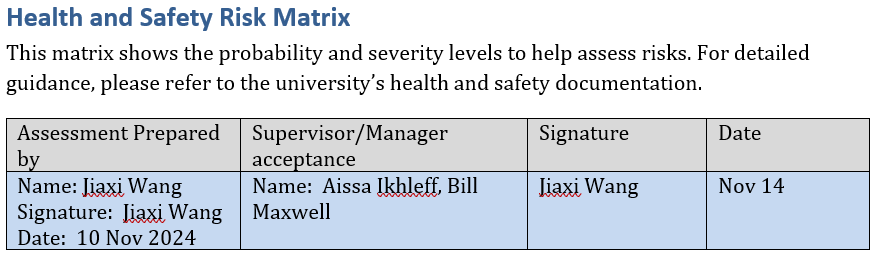
\includegraphics[width=0.85\textwidth]{Risk4.png}
    \caption{Risk Assessment – Automated Material Mover Project}
    \label{fig:risk_assessment}
\end{figure}
\FloatBarrier

\section{Recommendations/Conclusion}
Based off our initial studies, the URS created seems to be largely appropriate for this project however, we may need to make some minor refinements to better align it with the enhanced manoeuvrability and sustainability focus of our chosen design. This project should proceed as planned based off the information given in this report covering technical feasibility, cost effectiveness and environmental advantages of the proposed three-wheeled automated forklift. Our analysis confirm that the autonomous material mover will be able to provide not only an economical but also a sustainable solution for warehouse operations in the future, with a breakeven point compared to conventional forklifts of only 420 days after implementation. This design effectively balances performance, cost and sustainability making it the prefect choice for modern industrial automation needs.

\FloatBarrier

% -------------------------------------------------------------
% 6. Project Schedule
% -------------------------------------------------------------
\section{Project Schedule}

In order to plan out the schedule throughout the project, a Gantt Chart was created to plan out the hours worked every week, ensuring no tasks are ignored or missed out, giving them ample time to be completed. Additionally, leaving contingency hours caters for scope creep and any drastic changes that need to be made and also giving flexibility to change tasks and the hours put into them. The dynamic Gantt Chart in  figure \ref{fig:x}, made using Microsoft Excel, shows how complete each task is, and helps to visualise which tasks are on track, ahead or behind schedule. 

\begin{figure}[ht]
    \centering
    \begin{minipage}{0.45\linewidth}
        \centering
        \includegraphics[width=\linewidth]{BIGGER Gantt chart.png} % Replace with your Blender animation image
        \caption{Dynamic Project Gantt Chart}
        \label{fig:x}
    \end{minipage}
    \hspace{0.05\linewidth}
    \begin{minipage}{0.45\linewidth}
        \centering
        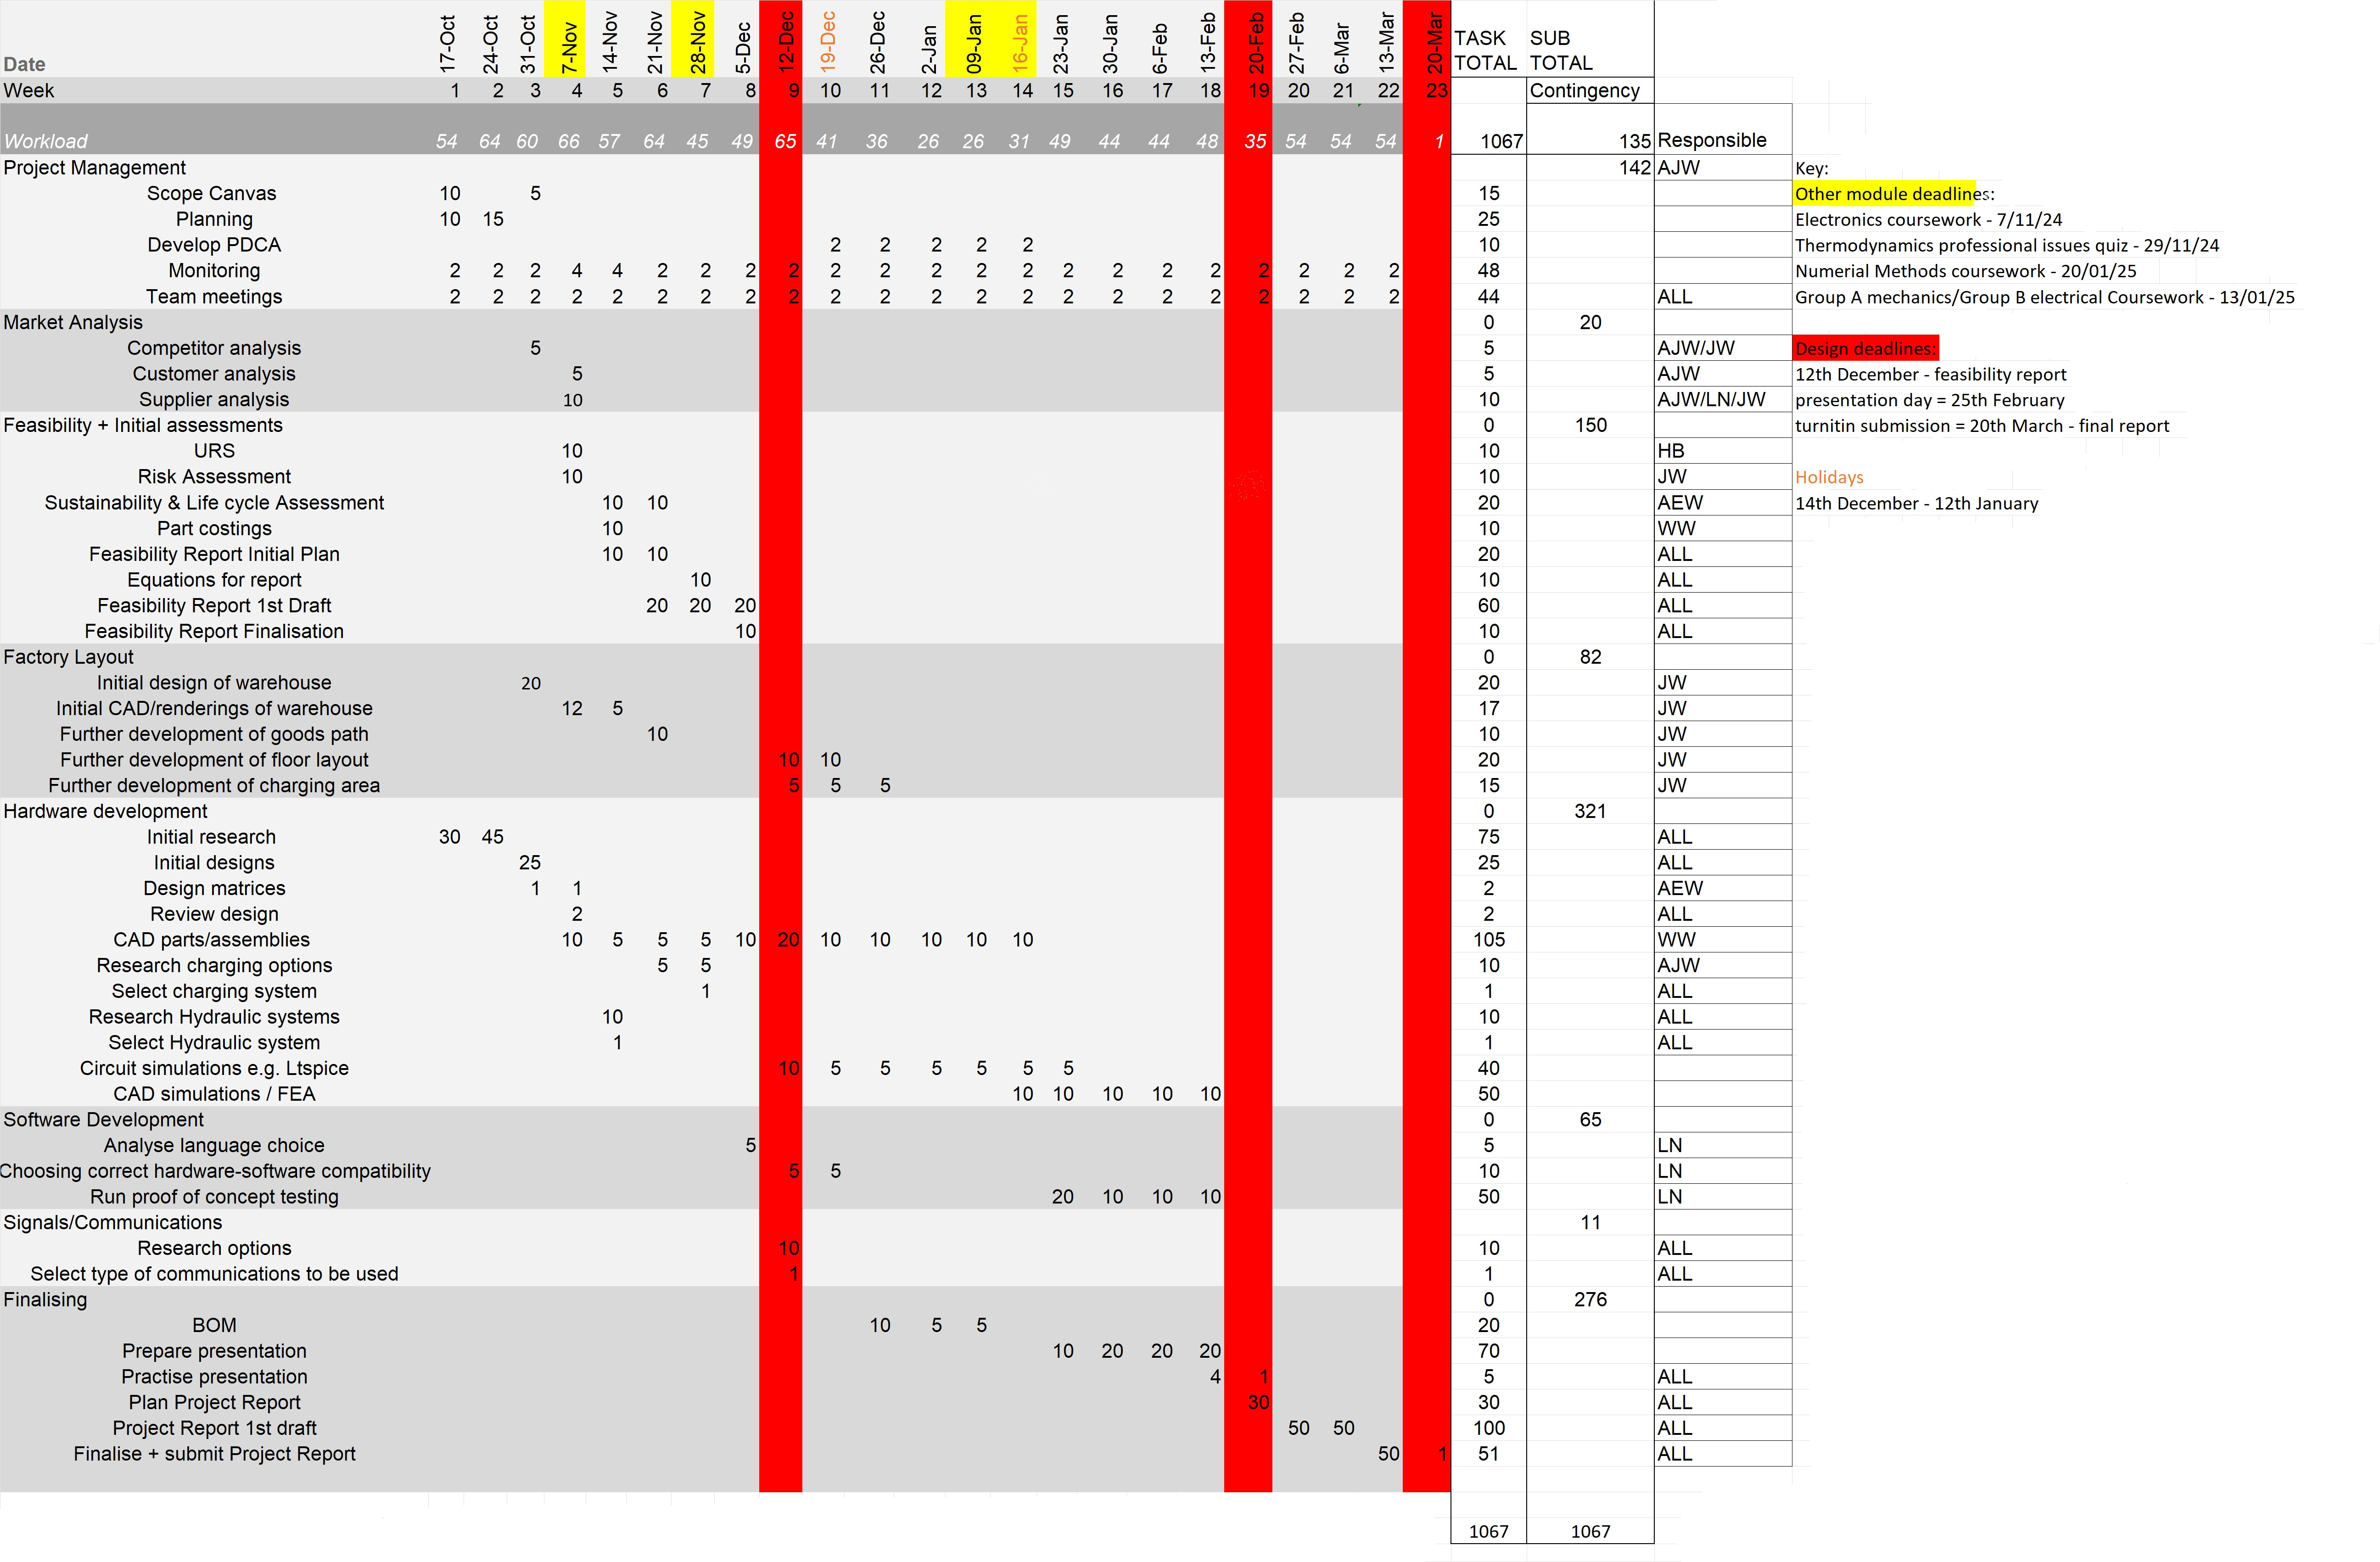
\includegraphics[width=\linewidth]{Gantt plan final.jpg}
        \caption{Planning Gantt Chart}
        \label{fig:y}
    \end{minipage}
\end{figure}
The planning Gantt Chart, figure \ref{fig:y}, showcases the weekly hours expected to be put into tasks and helps to ensure a balanced workload throughout the project. It also allows foresight for deadlines and other departmental commitments so that the workload can be planned around these accordingly. The majority of first term was planned around choosing a feasible design for the material mover and the research and drawings for this, as well as the factory layout the mover would work in. This provides a strong basis for the remainder of the project which focuses on CAD, software proof of concept and other simulations. This plan also allows for scope creep, having 135 contingency hours, and so means the project has ample time to be complete. 
\FloatBarrier
\begin{figure}[h!]
 \subsection{Meeting Minutes}
    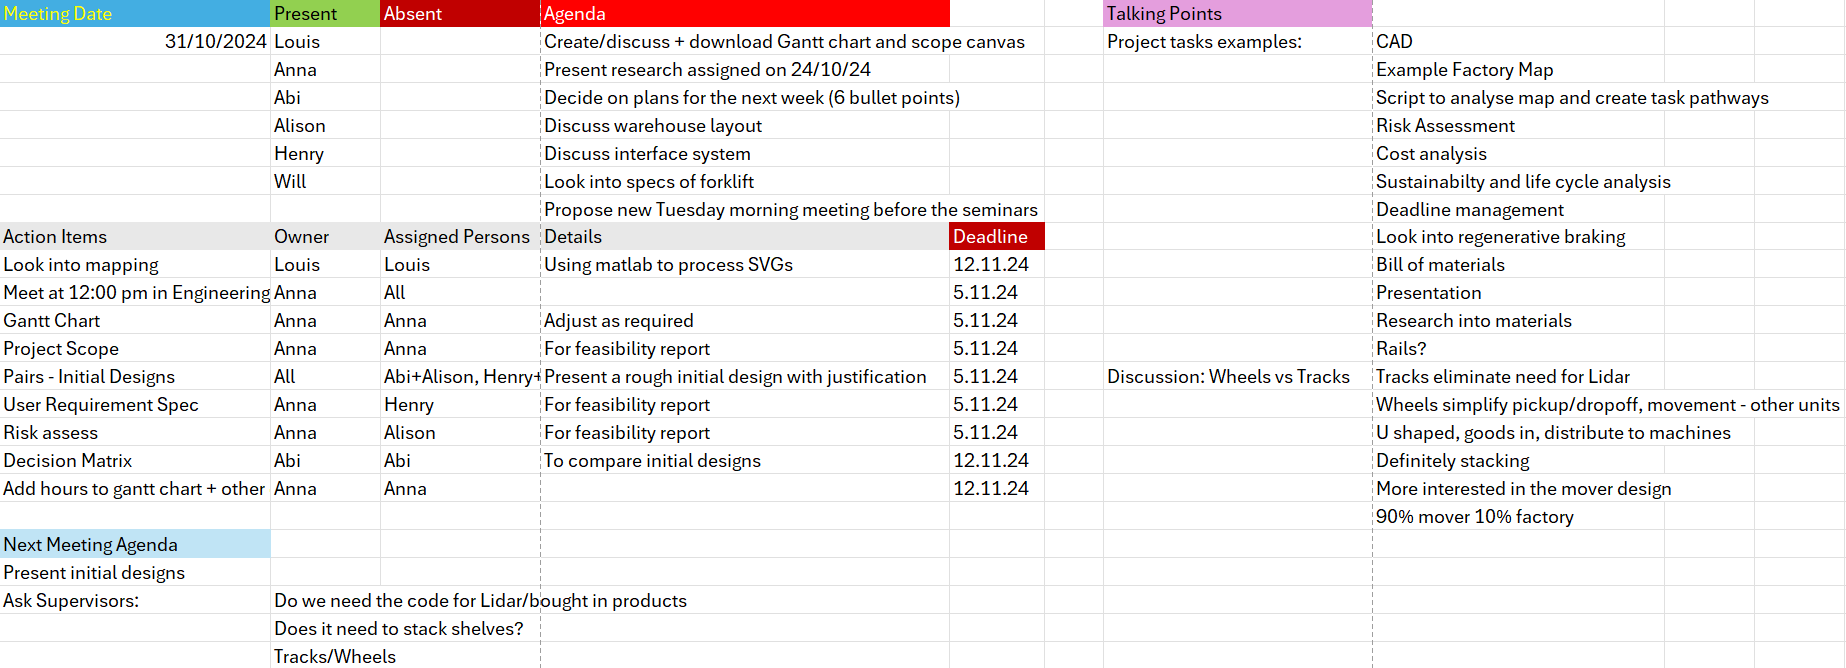
\includegraphics[width=1\textwidth]{HalloweenMinutes1.png}
    \caption{Meeting minutes from 31/10/24}
    \label{fig:x}
\end{figure}
  \FloatBarrier
Meeting minutes are a core component for the project management of this process. They are a detailed record of all discussions, decisions and assigned tasks. They are taken by the secretary every meeting, which is at least twice a week ensuring consistent and efficient collaboration. This ensures that all topics of discussion are covered and that appropriate tasks are assigned regularly, as well as allowing absent team members to catch up. Maintaining detailed minutes ensured that the whole team was aligned on priorities and deadlines as well as holding people accountable and reducing the risk of miscommunication.


\begin{thebibliography}{99}
\footnotesize
\setlength{\baselineskip}{0.8\baselineskip}

\bibitem{MathWorks}
MathWorks, “What Is SLAM (Simultaneous Localization and Mapping) – MATLAB \& Simulink,” \textit{uk.mathworks.com}.  
Available at: \url{https://uk.mathworks.com/discovery/slam.html} (accessed Nov. 20, 2024).
 

\bibitem{ToyotaForklifts}
Toyota Forklifts, “Automated Warehouse Trucks,” \textit{toyota-forklifts.co.uk}.  
Available at: \url{https://toyota-forklifts.co.uk/automated-solutions/automated-warehouse-trucks/} (accessed Nov. 20, 2024).

\bibitem{Forkify}
Forkify, “Forklift Cost Buyers Guide,” \textit{forkify.com}.  
Available at: \url{https://forkify.com/buyers-guide/forklift-cost/} (accessed Nov. 20, 2024).


\bibitem{LangleyShop}
Langley Shop, “Forklift Forks 100x40x1200 Class 2A,” \textit{langleyshop.co.uk}.  
Available at: \url{https://www.langleyshop.co.uk/product/forklift-forks-100x40x1200-class-2a/} (accessed Nov. 20, 2024).

\bibitem{CheckaTrade}
Checkatrade, “Electric Car Charger Installation Cost,” \textit{checkatrade.com}.  
Available at: \url{https://www.checkatrade.com/blog/cost-guides/electric-car-charger-installation-cost/} (accessed Nov. 20, 2024).

\bibitem{SalaryExpert}
Salary Expert, “Forklift Driver Salary in South Korea,” \textit{salaryexpert.com}.  
Available at: \url{https://www.salaryexpert.com/salary/job/forklift-driver/south-korea?form=MG0AV3} (accessed Nov. 20, 2024).

\bibitem{MordorIntelligence}
Mordor Intelligence, “Automated Material Handling Market,” \textit{mordorintelligence.com}.  
Available at: \url{https://www.mordorintelligence.com/industry-reports/automated-material-handling-market} (accessed Nov. 20, 2024).

\bibitem{GrandViewResearch}
Grand View Research, “Automated Guided Vehicle (AGV) Market,” \textit{grandviewresearch.com}.  
Available at: \url{https://www.grandviewresearch.com/industry-analysis/automated-guided-vehicle-agv-market} (accessed Nov. 20, 2024).

\bibitem{baker2023} T. Baker, ``5 Reason Why Structural Steel is Such a Sustainable Material,'' \textit{Baker Steel Trading}, 2023. [Online]. Available: \url{https://www.bakersteeltrading.co.uk/is-structural-steel-sustainable/}. [Accessed: Nov. 21, 2024].

\bibitem{eco2022} S. Co, ``We use ECO-FRIENDLY production techniques and technology,'' \textit{ENJOYING GO}, Sep. 21, 2022. [Online]. Available: \url{https://www.enjoycaster.com/en/solutions/product/eco-friendly-production}. [Accessed: Nov. 25, 2024].

\bibitem{ImperialTyres} 
``How is the tyre industry becoming more sustainable?,'' \textit{Imperial Tyres}, 2024. [Online]. Available: \url{https://www.imperialtyres.co.uk/blog/how-is-the-tyre-industry-becoming-more-sustainable/}. [Accessed: Nov. 21, 2024]

\bibitem{iso2330}
British Standards Institute, \textit{BS ISO 2330:2002: Fork-Lift Trucks. Fork Arms. Technical Characteristics and Testing}, 2002, \url{https://www.bsigroup.com/} (Accessed: December 6, 2024).

\bibitem{ForkDimensions}
Author Name, \textit{Fork Dimensions Reference}, Year, \url{https://www.azom.com/properties.aspx?ArticleID=965} (Accessed: December 6, 2024).



\bibitem{P. Hinz}
P. Hinz, “How Much Electricity does a Forklift Use per Hour?,” Adaptalift, Sep. 2021. \url{https://www.adaptalift.com.au/blog/how-much-electricity-does-a-forklift-use-per-hour }(accessed Nov. 25, 2024).

 \bibitem{mileway_hurworth_2024}
Mileway, “Hurworth Road, Newton Aycliffe Industrial Estate,” \url{https://mileway.com/properties/gb/portfolio/hurworth-road-newton-aycliffe-industrial-estate/} (accessed Dec. 2, 2024).
 
\bibitem{Pastor-Tella2024}
A. Pastor-Tella, ``AGV Cost Whitepaper,'' \textit{Wiferion}, 2024}.




\bibitem{crown2024}

Crown Equipment Corporation, \textit{Achieving Sustained Automated Forklift Performance}, 2024, \url{https://www.crown.com/en-us/blog/articles/automation/Achieving-Sustained-Automated-Forklift-Performance.html#:~:text=Fortunately%2C%20automated%20forklifts%20require%20much,on%20and%20within%20the%20vehicle.} (Accessed: December 2, 2024).

 \bibitem{agvnetwork2024}
AGV Network, \textit{Download Area}, 2024, \url{https://www.agvnetwork.com/download/download-area} (Accessed: December 6, 2024).
\bibitem{roboteq2024}
Roboteq, \textit{Ordering Online - Navigation Sensors}, 2024, \url{https://www.roboteq.com/ordering/ordering-online#navigation-sensors} (Accessed: December 6, 2024).

\bibitem{Baker} Baker, T. (2023). 5 Reason Why Structural Steel is Such a Sustainable Material. [online] Available at: \url{https://www.bakersteeltrading.co.uk/is-structural-steel-sustainable/} (Accessed 21. Nov, 2024).

\bibitem{Co} S. Co, “We use ECO-FRIENDLY production techniques and technology.,” ENJOYING GO, Sep. 21, 2022. Available at: \url{https://www.enjoycaster.com/en/solutions/product/eco-friendly-production} (Accessed Nov. 25, 2024).

\bibitem{Brake} Brake \& Front End. (2021). The Future Of Tires: Sustainable, Airless \& Connected. [online] Available at: \url{https://www.brakeandfrontend.com/the-future-of-tires-sustainable-airless-connected/} (Accessed 21. Nov, 2024).

\bibitem{Roos} D. Roos, “5 Green Methods of Transporting Goods,” HowStuffWorks, Aug. 29, 2012. Available at: \url{https://science.howstuffworks.com/environmental/green-science/5-green-methods-transporting-goods.htm} (Accessed Nov. 25, 2024).

\bibitem{Ashmore} J. Ashmore, “Container Operator BG Freight Line Launches Greenest Newbuild Vessels to Drive Sustainability,” Afloat.ie, May 08, 2024. Available at: \url{https://afloat.ie/port-news/port-and-shipping-news/item/63086-bg-freight-line-launches-new-vessels-to-drive-sustainability} (Accessed Nov. 25, 2024).
\bibitem{Toyota} Toyota Material Handling Europe, "Engine powered forklift datasheet", April 25, 2023. Available at: \url{https://media.toyota-forklifts.eu/published/22508_Original%20document_toyota%20mh.pdf} (Accessed Nov. 25, 2024).

 

\end{thebibliography}
 
 

% -------------------------------------------------------------
% LISTS OF FIGURES AND TABLES
% -------------------------------------------------------------
\section{Appendices}
\renewcommand{\listfigurename}{Figures}
\renewcommand{\listtablename}{Tables}
\listoffigures                                         % Add list of figures
\listoftables                                        % Add list of tables



\end{document}
